%%%%%%%%%%%%%%%%%%%%%%%%%%%%%%%%%%%%%%%%%%%%%%%%%%%%
%												   %
%	BIBLIOTECA									   %
%												   %
%	Novembro 2014								   %
%												   %
%	Angela Cardoso e Catarina Terra				   %
%   											   %	
%%%%%%%%%%%%%%%%%%%%%%%%%%%%%%%%%%%%%%%%%%%%%%%%%%%%

\documentclass[12pt,a4paper,reqno]{report}
\linespread{1.5}

\usepackage{amsfonts,amsmath,amssymb,indentfirst,mathrsfs,amscd}
\usepackage[mathscr]{eucal}
\usepackage[active]{srcltx} %inverse search
\usepackage{tensor}
\usepackage[utf8x]{inputenc}
\usepackage[portuges]{babel}
\usepackage[T1]{fontenc}
\usepackage{tikz}
\usepackage{graphicx}
\usepackage[numbers,square, comma, sort&compress]{natbib}
\numberwithin{figure}{section}
\numberwithin{equation}{section}
\usepackage{scalefnt}
\usepackage[top=3cm, bottom=3cm, left=2.5cm, right=2.5cm]{geometry}
\usepackage{comment} 
%\usepackage{tweaklist}
%\renewcommand{\itemhook}{\setlength{\topsep}{0pt}%
%	\setlength{\itemsep}{0pt}}
%\renewcommand{\enumhook}{\setlength{\topsep}{0pt}%
%	\setlength{\itemsep}{0pt}}
%\usepackage[colorlinks]{hyperref}
\usepackage{MnSymbol}
%\usepackage[pdfpagelabels,pagebackref,hypertexnames=true,plainpages=false,naturalnames]{hyperref}
\usepackage[naturalnames]{hyperref}
\usepackage{enumitem}
\usepackage{titling}
\newcommand{\subtitle}[1]{%
  \posttitle{%
    \par\end{center}
    \begin{center}\large#1\end{center}
    \vskip0.5em}%
}
\newcommand{\HRule}{\rule{\linewidth}{0.5mm}}

\usepackage[official]{eurosym}

\def\Cpp{C\raisebox{0.5ex}{\tiny\textbf{++}}}

\makeatletter
\def\@makechapterhead#1{%
  %%%%\vspace*{50\p@}% %%% removed!
  {\parindent \z@ \raggedright \normalfont
    \ifnum \c@secnumdepth >\m@ne
        \huge\bfseries \@chapapp\space \thechapter
        \par\nobreak
        \vskip 20\p@
    \fi
    \interlinepenalty\@M
    \Huge \bfseries #1\par\nobreak
    \vskip 40\p@
  }}
\def\@makeschapterhead#1{%
  %%%%%\vspace*{50\p@}% %%% removed!
  {\parindent \z@ \raggedright
    \normalfont
    \interlinepenalty\@M
    \Huge \bfseries  #1\par\nobreak
    \vskip 40\p@
  }}
\makeatother


\begin{document}

\input{./title.tex}

\tableofcontents

%%%%%%%%%%%%%%
% INTRODUCAO %
%%%%%%%%%%%%%%
\chapter{Introdução}

No âmbito da disciplina de Algoritmos e Estruturas de Dados, foi-nos proposto implementar em \Cpp{} uma aplicação que permita a gestão de uma biblioteca.

O sistema deve conter informações sobre livros, leitores, funcionários e empréstimos de livros. A aplicação também deve permitir registar e gerir os empréstimos efetuados na biblioteca, assim como toda a informação já referida.

Cada leitor não pode ter mais de 3 livros emprestados em simultâneo. Por casa dia de atraso o leitor incorre numa multa de 0,25\euro{} por dia na primeira semana e de 0,50\euro{} por dia nas semanas seguintes.

Um livro pode ser emprestado por um período máximo de 1 semana ou não pode ser emprestado.

Cada empréstimo é feito por um funcionário. Os funcionários podem ou não ser supervisores e cada supervisor é responsável por um ou mais funcionários, nunca por outro supervisor, devendo esta distribuição ser equilibrada.

Ao longo deste documento descreve-se a aplicação que desenvolvemos para gestão de um biblioteca.

%%%%%%%%%%%%%
% DESCRICAO %
%%%%%%%%%%%%%
\chapter{Descrição da Solução Implementada}

Para conter toda a informação de uma biblioteca, implementou-se a classe \textbf{Biblioteca}, que é constituída pelos seguintes vetores:
\begin{itemize}
\item \textit{livros} - todos os livros da biblioteca;
\item \textit{funcionarios} - todos os funcionários, incluindo os supervisores e o administrador;
\item \textit{leitores} - todos os leitores da biblioteca;
\item \textit{emprestimos} - todos os empréstimos da biblioteca;
\item \textit{utilizadores} - todos os utilizadores do sistema informático da biblioteca.
\end{itemize}

Com exceção dos utilizadores, quando um objeto é removido (por exemplo, no caso de devolução de um empréstimo), não desaparece, apenas é alterado para indicar que já não existe, sendo-lhe acrescentada a data de remoção. Assim, para a classe \textbf{Livro} (respectivamente, \textbf{Funcionario}, \textbf{Leitor}, \textbf{Emprestimo}) existe a subclasse \textbf{Livro\_old} (respectivamente, \textbf{Funcionario\_old}, \textbf{Leitor\_old}, \textbf{Emprestimo\_old}), para onde é enviado um livro (respectivamente, funcionário, leitor, empréstimo) quando é removido.

As classes \textbf{Livro}, \textbf{Funcionario}, \textbf{Leitor}, \textbf{Emprestimo} e \textbf{Utilizador} são subclasses da classe \textbf{Object}, que tem como único atributo o código de identificação \textbf{ID}.

O primeiro passo na utilização da aplicação é efetuar o login. Para isso é necessário indicar o ID e a password, sendo então determinado o tipo de acesso do utilizador, 0 se for administrador (gerente da biblioteca), 1 se for um supervisor e 2 se for um funcionário. \underline{ID}, \underline{password} e \underline{acesso} são atributos da classe \textbf{Utilizador}.

Uma das funções mais procuradas numa biblioteca é o empréstimo de livros a leitores. A classe \textbf{Emprestimo} faz a gestão dessas funções e tem como parâmetros um apontador para o livro do emprestimo, um apontador para o funcionario que fez o emprestimo, um apontador para o leitor do emprestimo, a data do emprestimo e um contador de emprestimos feitos na biblioteca (atuais e antigos).

Tal como a classe \textbf{Emprestimo}, as classes \textbf{Livro}, \textbf{Funcionario} e \textbf{Leitor}, também possuem contadores do numero dos seus objetos na biblioteca. Estes contadores são utilizados para permitir a atribuição automática de códigos de identificação a cada um destes objetos. Assim, se adicionamos um novo livro à biblioteca, por exemplo, e em toda a sua existência (atuais e antigos) a biblioteca teve 13 livros, o ID do novo livro será 14.

A classe \textbf{Livro} tem como atributos o \underline{titulo}, um vetor com os nomes dos \underline{autores}, o \underline{tema}, o \underline{ISBN}, a \underline{cota} do livro na biblioteca, o \underline{num\_paginas}, a \underline{edicao}, o booleano \underline{emprestado} (que é verdadeiro caso este esteja emprestado e a falso caso contrário) e, caso o livro esteja emprestado, a identificação do empréstimo do livro \underline{ID\_ep} e a \underline{data} do empréstimo.

Além dos atributos já referidos, o único atributo da classe \textbf{Funcionario} é o \underline{nome} do funcionário. A classe \textbf{Supervisor} é subclasse de \textbf{Funcionario} e tem como atributo adicional um vetor \underline{funcionarios\_sup} de apontadores para os funcionários supervisionados pelo supervisor. Uma vez que o número de funcionários supervisionados por cada supervisor deve ser equilibrado, a distribuição dos funcionários pelos supervisores é feita de forma automática, garantindo o equilíbrio, de cada vez que:
\begin{itemize}
	\item é adicionado um funcionário;
	\item é removido um funcionário ou supervisor;
	\item é promovido um funcionário a supervisor;
	\item é despromovido um supervisor a funcionário.
\end{itemize}

Existe ainda a classe \textbf{Administrador}, como subclasse de \textbf{Funcionario} (sem atributos adicionais). Apenas é adicionado um administrador à biblioteca, com o ID 0 e o nome Administrador. Este age como gerente da biblioteca, sendo o único que tem acesso total e que pode adicionar, remover, promover e despromover funcionários. É também o único que pode efetuar a manutenção dos utilizadores.

Além dos mencionados acima, os atributos da classe \textbf{Leitor} são o \underline{nome}, o \underline{telefone}, o \underline{email} e um vetor \underline{emprestimos\_leitor} com apontadores para os seus empréstimos.

A interação do utilizador com a aplicação é feita primariamente através de uma série de menus na consola, de seleção numérica. Uma sequência de opções nestes menus, conduz a uma função da classe \textbf{Biblioteca}, que por sua vez poderá chamar uma ou mais funções das restantes classes mencionadas. A gestão destes menus é feita na classe \textbf{Menu}, subclasse de \textbf{Biblioteca}, que como atributo adicional tem um \textbf{Utilizador\_online}, consoante o qual é determinado o tipo de acesso e as funções disponíveis.

Além das classes mencionadas, existem ainda várias classes onde estão parametrizadas as exceções a usar quando não existe um determinado objeto, tentamos adicionar um empréstimo a um leitor com 3 empréstimos, tentamos emprestar um livro já emprestado, tentamos remover um objeto ocupado (livro emprestado, por exemplo), tentamos utilizar um ficheiro que não existe, etc.

%%%%%%%%%%%%
% DIAGRAMA %
%%%%%%%%%%%%
\chapter{Diagrama de Classes UML}

\begin{center}

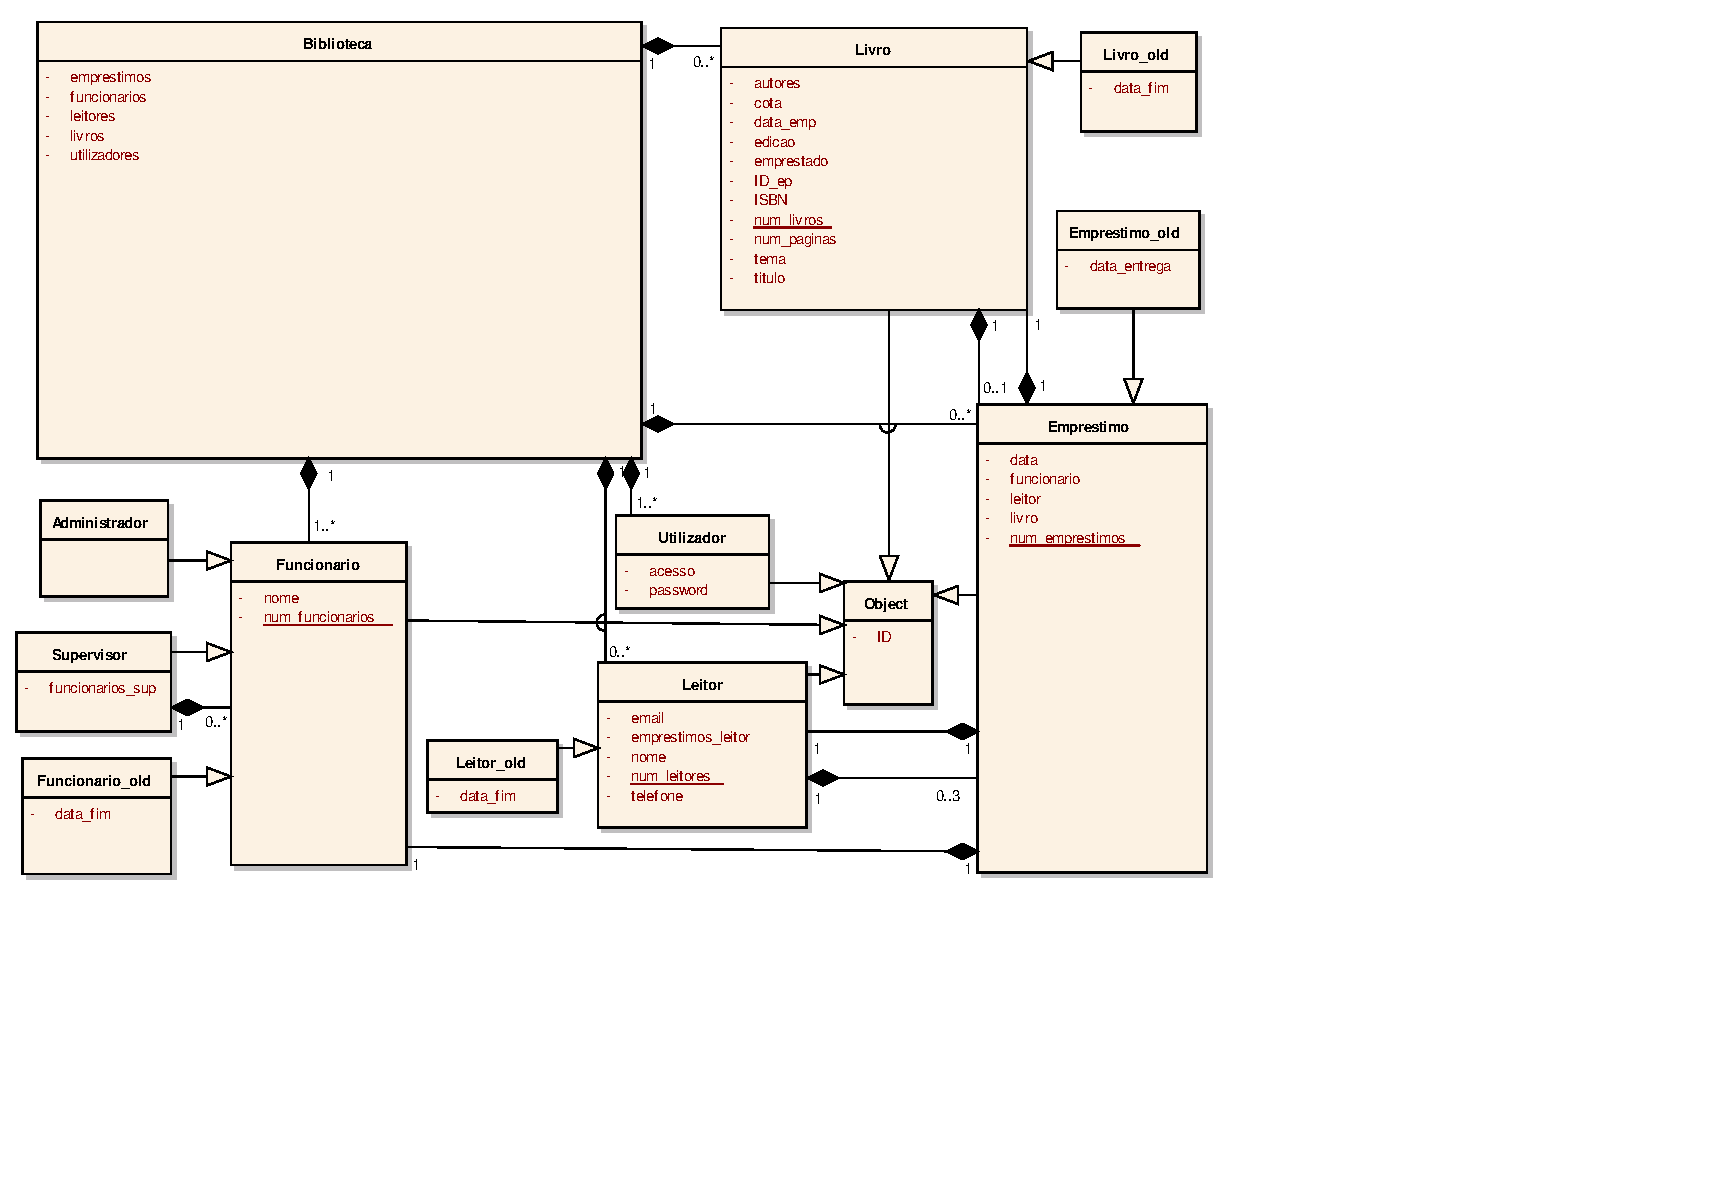
\includegraphics[width=14cm]{UML.jpg}

\end{center}

%%%%%%%%%%%%%%
% UTILIZACAO %
%%%%%%%%%%%%%%
\chapter{Casos de Utilização}

A aplicação para gestão de uma biblioteca construída permite registar informaticamente uma série de atividades relacionadas com o funcionamento normal de uma biblioteca.

\begin{enumerate}
  \item Consultas
  \begin{enumerate}[label*=\arabic*.]
    \item Livros
    \item Empréstimos
    \item Leitores
    \item Funcionários
    \item Supervisores
    \item Utilizadores
  \end{enumerate}
  \item Empréstimos
  \begin{enumerate}[label*=\arabic*.]
    \item Adicionar
    \item Devolver
    \item Consultar atrasos
    \item Consultar atrasos por leitor
    \item Consultar livros atrasados
    \item Consultar antigos
  \end{enumerate}
  \item Livros
  \begin{enumerate}[label*=\arabic*.]
    \item Consultar disponíveis
    \item Consultar emprestados
    \item Consultar por tema
    \item Consultar antigos
    \item Adicionar
    \item Remover
  \end{enumerate}
  \item Leitores
  \begin{enumerate}[label*=\arabic*.]
    \item Adicionar
    \item Remover
    \item Alterar
    \item Consultar antigos
  \end{enumerate}
  \item Funcionários
  \begin{enumerate}[label*=\arabic*.]
    \item Adicionar
    \item Remover
    \item Promover
    \item Despromover
    \item Consultar antigos
  \end{enumerate}
  \item Utilizadores
  \begin{enumerate}[label*=\arabic*.]
    \item Adicionar
    \item Remover
  \end{enumerate}
\end{enumerate}

A disponibilidade destas funções depende do nível de acesso do utilizador. De forma geral, um supervisor pode, além de todas as tarefas acessíveis a um funcionário, adicionar e remover livros e consultar informação sobre funcionários. O administrador é o único que pode fazer a manutenção dos funcionários e dos utilizadores.

%%%%%%%%%%%%%%%%
% DIFICULDADES %
%%%%%%%%%%%%%%%%
\chapter{Principais Dificuldades}

A maior dificuldade de implementação foi garantir a unicidade dos códigos de identificação para cada tipo de objeto. Isto porque uma vez tomada a decisão de automatizar a atribuição destes códigos, é necessário manter contadores do número de cada um dos objetos. Ora, ao retirar um objeto da biblioteca, da próxima vez que o programa for iniciado, será contado menos um objeto desse tipo e consequentemente poderia ser criado um novo objeto com ID igual ao do último objeto desse tipo.

Perante este problema, a primeira solução pensada foi guardar os contadores no final de cada utilização, em vez de voltar a contar os objetos ao ler os ficheiros no início de cada utilização. No entanto, uma vez que pelo menos o histórico de empréstimos faz todo o sentido guardar, a solução implementada passou por guardar histórico de praticamente todos os objetos da biblioteca. Esta alternativa é mais completa e mais próxima da realidade, uma vez que os sistemas informáticos habitualmente mantém histórico dos objetos que criam.

A restantes dificuldades prenderam-se com o desconhecimento de algumas das ferramentas utilizadas, como o Doxygen e o Enterprise Architect, assim como algum desconhecimento da linguagem \Cpp{}, nomeadamente a nível de exceções. A ajuda do Monitor Tiago Azevedo nestas questões, a sua orientação para lidar com polimorfismo e as várias funções de \Cpp{} por ele introduzidas, revelaram-se essenciais.

%%%%%%%%%%%%%%%%
% DISTRIBUICAO %
%%%%%%%%%%%%%%%%
\chapter{Distribuição de Trabalho Pelos Elementos do Grupo}

Mais do que a implementação e realização do trabalho propriamente ditas, houve várias dificuldades de gestão das tarefas e da participação de cada elemento do grupo.

Inicialmente, o grupo era composto por três elementos, além das autoras, a colega Maria Miranda fazia parte do grupo e participou na reunião inicial assim como numa das reuniões posteriores. Foi a Maria que sugeriu que os livros tivessem temas, que os supervisores tivessem nível de acesso superior ao dos funcionários, que se separassem os ficheiros de código consoante as classes e que se usassem ciclos for sempre que possível, em vez de ciclos while.

A distribuição de tarefas da primeira reunião foi a seguinte:
\begin{itemize}
	\item Ângela - implementação das classes ``primárias'';
	\item Catarina - construção dos ficheiros de texto com a informação e das funções para ler e escrever esses mesmos ficheiros;
	\item Maria - criação dos menus e de toda a interação entre o utilizador e a aplicação.
\end{itemize}

A disponibilidade dos elementos do grupo para o trabalho não foi claramente a mesma e como tal a Ângela, uma vez terminadas as suas tarefas, começou por colaborar com a Catarina nas dela, tendo para isso sido aproveitadas reuniões a que a Maria não compareceu. Quando se aproximou a data de entrega, dado que a Maria não disponibilizou a sua parte, a Ângela avançou com os menus, tendo comunicado antecipadamente que o iria fazer. No final, ainda sem disponibilizar o seu código, a Maria insistiu que o queria utilizar e como tal acabou por decidir separar-se do grupo. Entretanto, a documentação do trabalho foi dividida irmamente pelos elementos restantes.

\chapter{Conclusão}

Obviamente a experiência e o resultado final teriam sido mais positivos para todos os elementos do grupo inicial, caso as pessoas pudessem todas colaborar de forma equilibrada. No entanto, este desenrolar contribuiu para a nossa aprendizagem e da próxima vez certamente será melhor.

O trabalho em si foi muito interessante e a aquisição de conhecimentos foi particularmente intensa. Mais do que a frequência das aulas e até mesmo a realização dos testes, este tipo de trabalho ajuda a sedimentar as várias noções introduzidas na disciplina.

Naturalmente, quem termina uma tarefa desta natureza já não é a mesma pessoa que a iniciou. Se fosse feito novamente, certamente sofreria várias alterações.

\end{document}
